\documentclass{assignment}

\course{ECO 120-04}
\name{Lucas Reddinger}
\date{Friday 7 October 2022}
\doctitle{Assignment 5 Solutions}

\begin{document}
\RaggedRight

\beginsolutions{}

\section{The U.S.~market for used cars}

\begin{enumerate}

\item Depict the U.S.~market for used cars in equilibrium with a supply and demand model. Label the curves as $S$ and $D$, equilibrium price as $p^*_1$, equilibrium quantity as $q^*_1$, and axes as appropriate.

\begin{solution}
\begin{center}
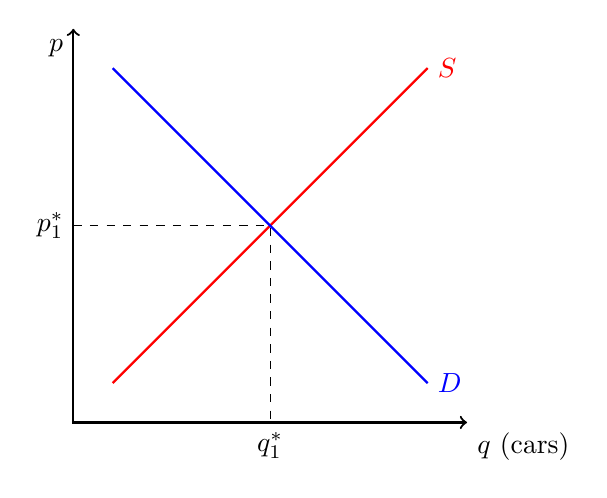
\begin{tikzpicture}[scale=0.5]
\draw[thick,<->] (0,10) node[below left]{$p$}--(0,0)--(10,0) node[below right]{$q$ (cars)};
\draw[thick,red] (1,1)--(9,9) node[right]{$S$};
\draw[thick,blue] (1,9)--(9,1) node[right]{$D$};
\draw[dashed] (0,5) node[left]{$p^*_1$} --(5,5) --(5,0) node[below]{$q^*_1$};
\end{tikzpicture}
\end{center}
\vspace{-12pt}
\end{solution}

\item Suppose supply chain disruptions significantly reduce the availability of cars. Appropriately depict the new market-clearing equilibrium (e.g., prices, quantities, curves) using subscripts of 2.

\begin{solution}
Supply of used cars in the U.S.~has decreased. In supply and demand diagrams, a decrease is represented by an inward shift (to the left).

\begin{center}
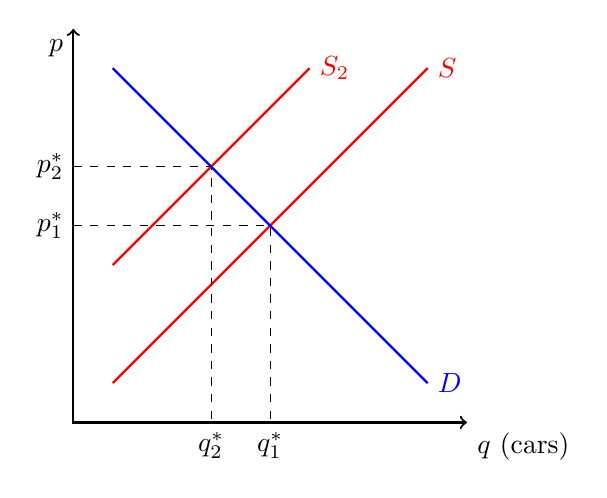
\begin{tikzpicture}[scale=0.5]
\draw[thick,<->] (0,10) node[below left]{$p$}--(0,0)--(10,0) node[below right]{$q$ (cars)};
\draw[thick,red] (1,1)--(9,9) node[right]{$S$};
\draw[thick,red] (1,4)--(6,9) node[right]{$S_2$};
\draw[thick,blue] (1,9)--(9,1) node[right]{$D$};
\draw[dashed] (0,5) node[left]{$p^*_1$} --(5,5) --(5,0) node[below]{$q^*_1$};
\draw[dashed] (0,6.5) node[left]{$p^*_2$} --(3.5,6.5) --(3.5,0) node[below]{$q^*_2$};
\end{tikzpicture}
\end{center}
\vspace{-12pt}
\end{solution}

\item What type of market is this---a factor market or a product market?

\begin{solution}
\emph{Complete answer:} A product market.

Used cars are generally demanded by household consumers, making them a product. Factors are bought by firms, whereas products are bought by households.
\end{solution}

\item What entities does the demand curve represent?

\begin{solution}
Any entities who may purchase (demand) used cars---most likely these are household consumers.
\end{solution}

\item What entities does the supply curve represent?

\begin{solution}
Any entities who may sell used cars. Used car dealers are \emph{firms} who sell used cars.

Note that some households may sell used cars. In general, however, the supply-side of a product market consists of firms, and the demand-side of a product market consists of households.
\end{solution}

\item Do you know whether $q^*_2$ is higher than, lower than, or the same as $q^*_1$?

\begin{solution}
\emph{Complete answer:} $q^*_2 < q^*_1$.

The equilibrium quantity of used cars traded has decreased. This makes intuitive sense, as fewer cars are now being supplied.
\end{solution}

\item Do you know whether $p^*_2$ is higher than, lower than, or the same as $p^*_1$?

\begin{solution}
\emph{Complete answer:} $p^*_2 > p^*_1$.

The equilibrium price of used cars traded has increased. This makes intuitive sense, as fewer cars are now being supplied. When something becomes more scarce, its price increases.
\end{solution}

\end{enumerate}

\section{The U.S.~labor market}

\begin{enumerate}

\item Depict the U.S.~labor market in equilibrium with a supply and demand model. Label the curves as $S$ and $D$, equilibrium price as $w^*_1$, equilibrium quantity as $L^*_1$, and axes as appropriate.

\begin{solution}
\begin{center}
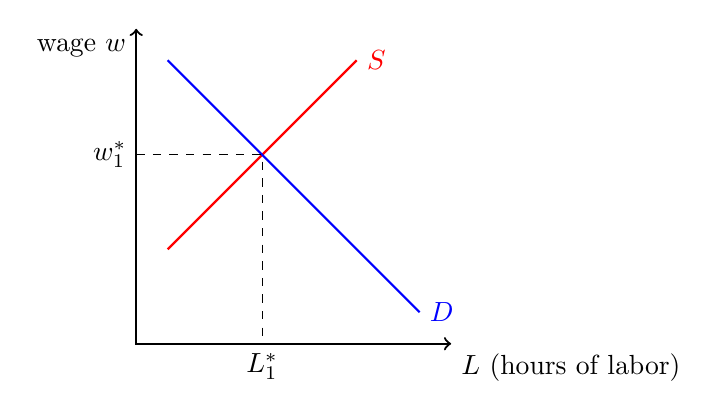
\begin{tikzpicture}[scale=0.4]
\draw[thick,<->] (0,10) node[below left]{wage $w$}--(0,0)--(10,0) node[below right]{$L$ (hours of labor)};
\draw[thick,red] (1,3)--(7,9) node[right]{$S$};
\draw[thick,blue] (1,9)--(9,1) node[right]{$D$};
\draw[dashed] (0,6) node[left]{$w^*_1$} --(4,6) --(4,0) node[below]{$L^*_1$};
\end{tikzpicture}
\end{center}
\vspace{-12pt}
\end{solution}

\item Suppose that due to COVID-19 cases declining, more people want to work. Appropriately shift any curves, labeled with subscripts of 2.

\begin{solution}
Supply of labor in the U.S.~has increased. In supply and demand diagrams, an increase is represented by an outward shift (to the right).

\begin{center}
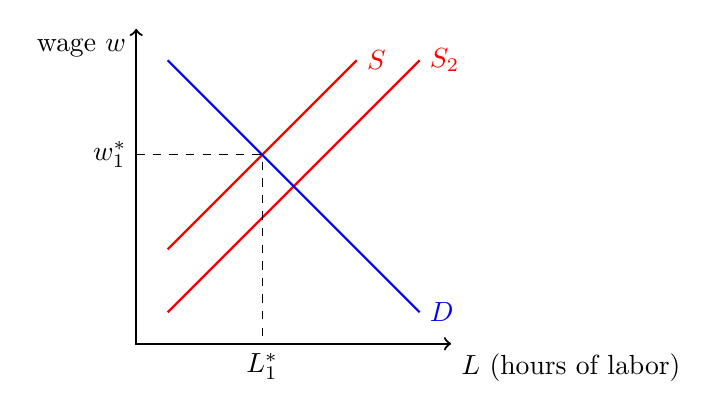
\begin{tikzpicture}[scale=0.4]
\draw[thick,<->] (0,10) node[below left]{wage $w$}--(0,0)--(10,0) node[below right]{$L$ (hours of labor)};
\draw[thick,red] (1,3)--(7,9) node[right]{$S$};
\draw[thick,red] (1,1)--(9,9) node[right]{$S_2$};
\draw[thick,blue] (1,9)--(9,1) node[right]{$D$};
\draw[dashed] (0,6) node[left]{$w^*_1$} --(4,6) --(4,0) node[below]{$L^*_1$};
\end{tikzpicture}
\end{center}
\vspace{-12pt}
\end{solution}

\item Because the demand for consumer goods is strong, firms want to hire more workers. Appropriately shift any curves, labeled with subscripts of 3.

\begin{solution}
Demand of labor in the U.S.~has increased. In supply and demand diagrams, an increase is represented by an outward shift (to the right).

\begin{center}
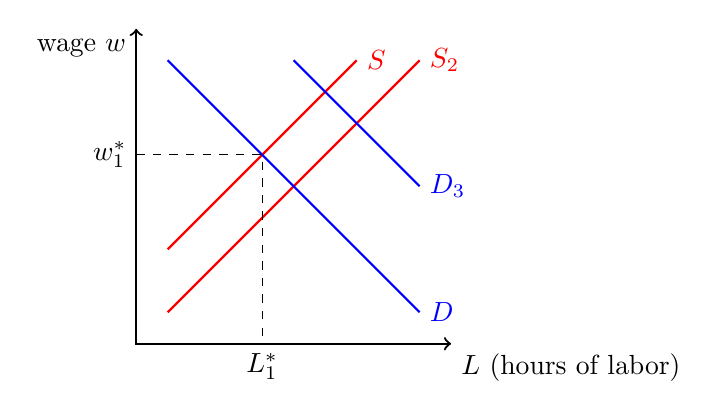
\begin{tikzpicture}[scale=0.4]
\draw[thick,<->] (0,10) node[below left]{wage $w$}--(0,0)--(10,0) node[below right]{$L$ (hours of labor)};
\draw[thick,red] (1,3)--(7,9) node[right]{$S$};
\draw[thick,red] (1,1)--(9,9) node[right]{$S_2$};
\draw[thick,blue] (1,9)--(9,1) node[right]{$D$};
\draw[thick,blue] (5,9)--(9,5) node[right]{$D_3$};
\draw[dashed] (0,6) node[left]{$w^*_1$} --(4,6) --(4,0) node[below]{$L^*_1$};
\end{tikzpicture}
\end{center}
\vspace{-12pt}
\end{solution}

\item Given this tandem of changes to supply and demand, please label the new equilibrium wage as $w^*_3$ and equilibrium quantity of labor traded as $L^*_3$.

\begin{solution}
\begin{center}
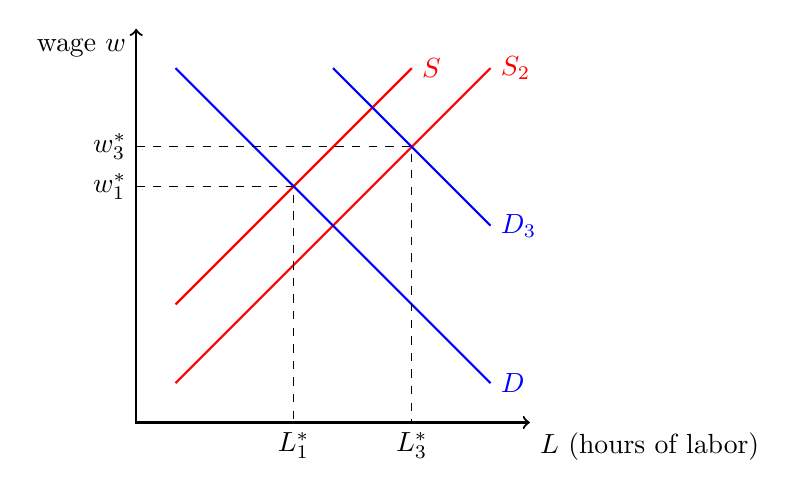
\begin{tikzpicture}[scale=0.5]
\draw[thick,<->] (0,10) node[below left]{wage $w$}--(0,0)--(10,0) node[below right]{$L$ (hours of labor)};
\draw[thick,red] (1,3)--(7,9) node[right]{$S$};
\draw[thick,red] (1,1)--(9,9) node[right]{$S_2$};
\draw[thick,blue] (1,9)--(9,1) node[right]{$D$};
\draw[thick,blue] (5,9)--(9,5) node[right]{$D_3$};
\draw[dashed] (0,6) node[left]{$w^*_1$} --(4,6) --(4,0) node[below]{$L^*_1$};
\draw[dashed](0,7) node[left]{$w^*_3$} --(7,7) --(7,0) node[below]{$L^*_3$};
\end{tikzpicture}
\end{center}
\vspace{-12pt}
\end{solution}

\item What type of market is this---a factor market or a product market?

\begin{solution}
\emph{Complete answer:} It is a factor market.

Labor is considered a factor market, as it is one of two factors of production. Firms use two factors---capital and labor---to produce goods.
\end{solution}

\item What entities does the demand curve represent?

\begin{solution}
\emph{Complete answer:} Firms.

Firms demand labor and pay wages (which is the price of hourly labor).
\end{solution}

\item What entities does the supply curve represent?

\begin{solution}
\emph{Complete answer:} Households.

Households supply labor and are paid wages for labor supplied.
\end{solution}

\item Considering the two changes in tandem, has labor traded increased, decreased, or stayed the same? Or do you not have enough information to determine this overall effect? That is, do you know whether $L^*_3$ is higher than, lower than, or the same as $L^*_1$?

\begin{solution}
Each of the two changes increased labor traded. Therefore the net affect on equilibrium labor traded must be positive.
\end{solution}

\item Considering the two changes in tandem, has the wage increased, decreased, or stayed the same? Or do you not have enough information to determine this overall effect? That is, do you know whether $w^*_3$ is higher than, lower than, or the same as $w^*_1$?

\begin{solution}
\emph{Complete answer:} The overall change in equilibrium wage is ambiguous.

The increase in supply lowered wages. The increase in demand raised wages. Because one change had a positive effect on wages while the other had a negative effect, the net effect is ambiguous. Consider the alternate depiction below.

\begin{center}
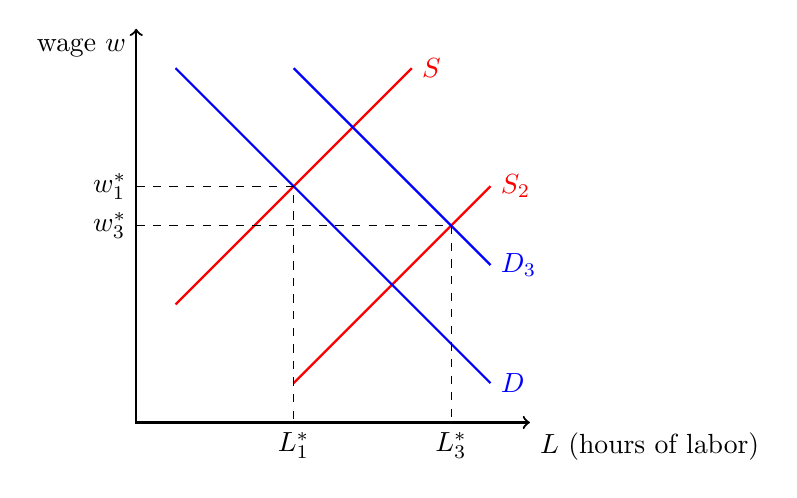
\begin{tikzpicture}[scale=0.5]
\draw[thick,<->] (0,10) node[below left]{wage $w$}--(0,0)--(10,0) node[below right]{$L$ (hours of labor)};
\draw[thick,red] (1,3)--(7,9) node[right]{$S$};
\draw[thick,red] (4,1)--(9,6) node[right]{$S_2$};
\draw[thick,blue] (1,9)--(9,1) node[right]{$D$};
\draw[thick,blue] (4,9)--(9,4) node[right]{$D_3$};
\draw[dashed] (0,6) node[left]{$w^*_1$} --(4,6) --(4,0) node[below]{$L^*_1$};
\draw[dashed](0,5) node[left]{$w^*_3$} --(8,5) --(8,0) node[below]{$L^*_3$};
\end{tikzpicture}
\end{center}
\vspace{-12pt}
\end{solution}

\end{enumerate}

\section{The U.S.~loanable funds market}

\begin{enumerate}

\item Depict the loanable funds market in equilibrium with a supply and demand model. Label the curves as $S$ and $D$, equilibrium rate as $r^*_1$, equilibrium quantity as $Q^*_1$, and axes as appropriate.

\begin{solution}
\begin{center}
\begin{tikzpicture}[scale=0.5]
\draw[thick,<->] (0,10) node[below left]{interest rate $r$}--(0,0)--(10,0) node[below right]{$Q$ (loanable funds)};
\draw[thick,red] (1,3)--(7,9) node[right]{$S$};
\draw[thick,blue] (1,9)--(9,1) node[right]{$D$};
\draw[dashed] (0,6) node[left]{$r^*_1$} --(4,6) --(4,0) node[below]{$Q^*_1$};
\end{tikzpicture}
\end{center}
\vspace{-12pt}
\end{solution}

\item Suppose that many investors divest from Russia, moving funds to the U.S. Appropriately depict the new market-clearing equilibrium (e.g., interest rates, quantities, curves) using subscripts of 2.

\begin{solution}
Investors (households) have stopped supplying loanable funds to Russian firms; they now instead supply more loanable funds to U.S.~firms.

\begin{center}
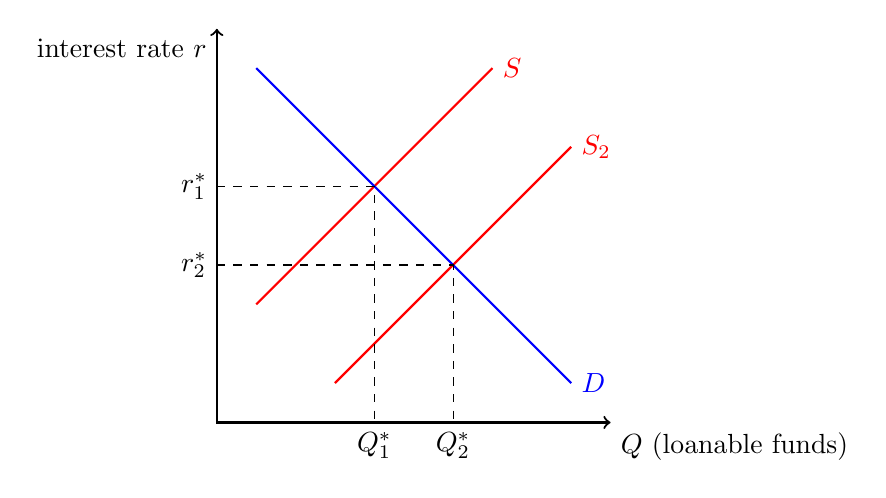
\begin{tikzpicture}[scale=0.5]
\draw[thick,<->] (0,10) node[below left]{interest rate $r$}--(0,0)--(10,0) node[below right]{$Q$ (loanable funds)};
\draw[thick,red] (1,3)--(7,9) node[right]{$S$};
\draw[thick,red] (3,1)--(9,7) node[right]{$S_2$};
\draw[thick,blue] (1,9)--(9,1) node[right]{$D$};
\draw[dashed] (0,6) node[left]{$r^*_1$} --(4,6) --(4,0) node[below]{$Q^*_1$};
\draw[dashed] (0,4) node[left]{$r^*_2$} --(6,4) --(6,0) node[below]{$Q^*_2$};
\end{tikzpicture}
\end{center}
\end{solution}

\item Has the market-clearing interest rate increased, decreased, or stayed the same?

\begin{solution}
\emph{Complete answer:} The equilibrium interest rate has decreased.

This makes intuitive sense because more loanable funds are now available in the U.S. When something becomes less scarce, its price decreases.
\end{solution}

\item What type of market is this---a factor market or a product market?

\begin{solution}
\emph{Complete answer:} It is a factor market.

The market for loanable funds is considered a factor market, because loanable funds are one of two factors of production. Firms use factors of production---capital and labor---to produce goods. Loanable funds are a source of capital.
\end{solution}

\item What entities does the demand curve represent?

\begin{solution}
\emph{Complete answer:} Firms.

Firms borrow money to acquire and maintain equipment, land, and other property, all of which are capital.
\end{solution}

\item What entities does the supply curve represent?

\begin{solution}
\emph{Complete answer:} Households.

When households save money, they lend funds to firms. One example of this is retail banking; households deposit money in a savings account, and banks lend this money to firms.
\end{solution}

\end{enumerate}

\end{document}
